\chapter{Control}

\section{Conceptos básicos del control clásico}

\subsection{Análisis de error}


En un sistema de realimentación no unitaria podemos considerar el error 

\begin{equation*}
e(t) = r(t) - y(t)
\end{equation*}

en donde la señal de referencia es la señal de salida $y(t)$ está siguiendo, cuando el sistema tiene realimentación unitaria.

El error en estado estavble es

\begin{equation*}
e_{ss} = \lim_{t \to \infty} e(t)
\end{equation*}


\begin{figure}[H]
    \centering
    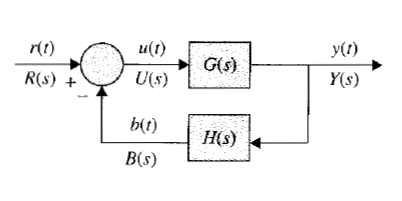
\includegraphics{Control/control_errorf2.png}
\end{figure}

en general si la realimentación es no unitaria, la señal $u(t)$ puede ya no será el error del sistema. Si el propósito del sistema es hacer que la salida siga a la referencia tan cerca como sea posible, y que las funciones de transferencia sean 




\begin{figure}[H]
    \centering
    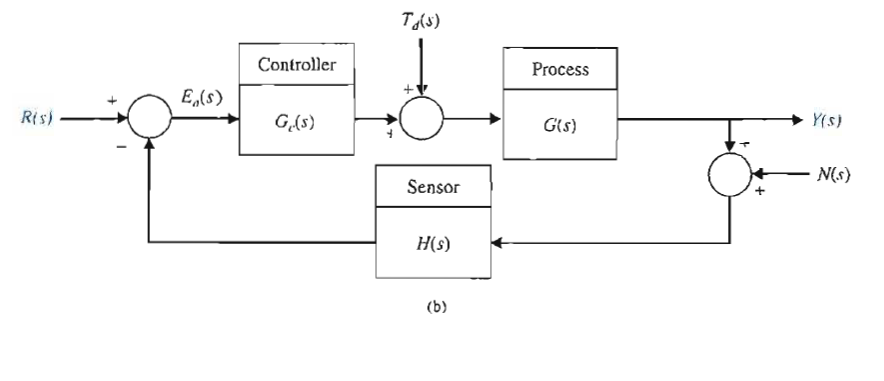
\includegraphics[scale=0.5]{Control/control_errorf1.png}
\end{figure}


El sistema de control de lazo cerrado mostrado en la figura anterior tiene tres entradas $R_(s)$, $T_d(s)$, y $N(s)$ y una salida. Las entradas $T(s)$ y $N(s)$ son señales de perturbaciones y de ruido respectivamente. Se define el error de seguimiento como

\begin{equation*}
E(s) = R(s) - Y(s)
\end{equation*}

Consideremos una realimentación unitaria, esto es $H(s) = 1$. Analizando este sistema de control encontramos que la salida del sistema está dada por

\begin{equation*}
Y(s) = R_(s) \frac{C(s)G(s)}{1 + C(s)G(s)} + T_d(s) \frac{G(s)}{1 + C(s)G(s)} - N(s) \frac{C(s)G(s)}{1 + C(s)G(s)}
\end{equation*}

como $E(s) = R(s) - Y(s)$, tenemos que, restando a $R(s)$ la expresión anterior

\begin{eqnarray*}
E(s) = \frac{1}{1 + C(s)G(s)}R(s) - \frac{G(s)}{1 + C(s)G(s)} T_d(s) + \frac{C(s)G(s)}{1 + C(s)G(s)} N(s)
\end{eqnarray*}

Llamemos a $L(s)=C(s)G(s)$ la función de lazo, esta función es importante en el análisis de sistemas de control. En términos de $L(s)$, la función de error se escribe:

\begin{equation*}
E(s) = \frac{1}{1+L(s)} R(s) - \frac{G(s)}{1+ L(s)}T_d(s) + \frac{L(s)}{1+L(s)}
\end{equation*}

Llamemos ahora a la función $F(s) = 1 + L(s)$ y definamos la función de sensiblildad como

\begin{equation*}
S(s) = \frac{1}{F(s)} = \frac{1}{1+L(s)}
\end{equation*}

y de manera similar definamos la función complementaria de sensibilidad como

\begin{equation*}
C_c(s) = \frac{L(s)}{1+L(s)}
\end{equation*}

Podemos escribir la función de error como

\begin{equation*}
E(s) = S(s) R(s) - S(s) G(s) T_d(S) + C_c(s) N(s)
\end{equation*}

vemos que para poder minimizar el error dada una función de transferencia $G(s)$, necesitamos que las funciones $S(s)$ y $C_c(s)$ sean muy pequeñas. (CONTINUAR LIBRO DORF PAG 215)


\section{Introducción y enfoques del control óptimo robusto}

\subsection{Estabilidad}

Para un sistema no lineal 

\begin{equation*}
    \dot{x} = A(x)
\end{equation*}

Donde $x \in \mathbb{R}^{n}$ y la función $A:\mathbb{R}^{n} \rightarrow \mathbb{R}^{n}$ es no lineal. Si $A(0) = 0$, el punto de equilibrio $x_0=0$ es asintóticamente estable si existe una vecindad de $x_0=0$ tal que si el sistema inicia en la vecindad, entonces su trayectoria converge al punto de equilibrio $x_0=0$ cuando $t \to \infty$.

Si el sistema es no lineal, determinar la estabilidad no es tarea sencilla. Una forma es con el enfoque de Lyapunov; una función de Lyapunov se define a partir de un sistema, esta función puede ser vista como una función de energía para el sistema. Esta función debe tener una propiedad de que su valor es cero en el origen y positiva en los demás lugares. Se asume también que la dinámica del sistema es tal que la energía del sistema es monótonamente decreciente con el tiempo y eventualmente llega a cero. Entonces las trayectorias del sistema no tienen otro lugar al cual dirigirse que no sea el origen. Por lo tanto el sistema es asintóticamente estable. Esta función generalizada de energía se denomina función de Lyapunov. \\

Por otro lado, para un sistema LTI $\dot{x}=Ax$, la estabilidad está dada por su ecuación característica.

\subsection{Control Óptimo}

Luego de estabilizar un sistema, lo siguiente que se quiere es optimizar el desempeño del sistema. Se formula el problema de control óptimo para un sistema general no lineal

\begin{equation*}
    \dot{x} = f(x,u)
\end{equation*}

y se requiere minimizar una función de costo

\begin{equation*}
    J(x,t) = \int_{t}^{t_f} L(x,u) d \tau
\end{equation*}

la función $L(x,u)$ caracteriza el objetivo de costo.\\

La solución del problema de control óptimo se deriva del principio de optimización, el cual establece que si un control es óptimo desde un estado inicial, entonces debe satisfacer la siguiente propiedad: luego de cualquier periodo inicial, el control del sistema para el periodo restante debe ser también óptimo con respecto al estado resultante del control en el periodo inicial. Aplicando el principio de optimización al problema de control óptimo, se puede derivar la ecuación Hamilton-Jacobi-Bellman que debe ser satisfecha por cualquier solución de controlador. \\

No siempre es sencillo resolver la ecuación Hamilton-Jacobi-Bellman, especialmente para sistema no lineales. Sin embargo, si el sistema es lineal y la función de costo es cuadrática, eso es

\begin{equation*}
    \dot{x} = A x + B u
\end{equation*}
\begin{equation*}
    J(x,t) = \int_{t}^{\infty} (x^TQ x+u^{T}R u)d \tau
\end{equation*}

Entonces dicha ecuación complicada se reduce a la siguiente ecuación de Riccati

\begin{equation*}
    S A + A^T S + Q - S B R^{-1} B^{T} S = 0
\end{equation*}

Al resolver la ecuación anterior de Riccati, para $S$, podemos obtener la solución para la señal de control:

\begin{equation*}
    u^{*} = - R^{-1} B^{T} S x
\end{equation*}

El anterior es el problema de control mediante regulador lineal cuadrático (LQR). El problema dual al regulador LQR es el de diseñar un observador óptimo, se denomina filtro de Kalman.

\subsection{Enfoque de control óptimo}

El sistema a ser controlado se describe por la siguiente forma

\begin{equation*}
    \dot{x}A(p)x + B u
\end{equation*}

Donde $p$ representa la incertidumbre. El objetivo es diseñar un estabilizador de realimentación de estados del sistema para todas las incertidumbres posibles $p$. La solución para este problema de control robusto depende de si la incertidumbre satisface una condición de coincidencia, lo cual requiere que la incertidumbre esté dentro de un rango dado por $B$. Si la incertidumbre satisface la condición de coincidencia, entonces la solución al problema de control siempre existirá y podrá obtenerse fácilmente mediante un regulador LQR. El problema LQR se obtiene incluyendo los límites de la incertidumbre en el funcional de costo.

\section{Análisis Lineal}

Uno de los puntos de vistas que prevalecen en el estudio de los sistemas y señales es aquel en el que un sistema dinámico se ve como un mapeo entre funciones de entrada y de salida. Este concepto subraya la gran mayoría de tratamiento de señales, comunicaciones y control. Aunque una perspectiva analítica funcional se utiliza de manera implícita en estas áreas, la maquinaria asociada no se usa directamente de manera típica para el estudio de sistemas dinámicos. Sin embargo, al incorporarse herramientas de análisis (como espacios de funciones, operadores) en este marco conceptual, surgen métodos de importancia clave para el estudio de sistemas. En particular, las normas de operadores provee una forma natural de cuantificar el "tamaño" de un sistema, el cual es un requerimiento fundamental para la teoría cuantitativa de incertidumbre de un sistema y aproximación de modelos.

En esta sección se verán algunos de los conceptos básicos del análisis que son requeridos para el desarrollo de la teoría de control robusto. Esto involucra el ensamble de algunas definiciones, con algunos ejemplos y presentando las propiedades importantes. 

\subsection{Espacios normados y productos internos}

El concepto matemático más importante en el curso de teoría de control robusto es el de espacio normado, el cual se usará continuamente como instrumento de medición tanto de señales como de sistemas.

\subsubsection{Def} Una norma $||\cdot||$ en un espacio vectorial $\mathcal{V}$ es un mapeo $\mathcal{V} \to [ 0,\infty)$ el cual satisface para cada $v \in \mathcal{V}$ las siguientes propiedades:

\begin{itemize}
    \item $|| v ||_{\mathcal{V}} = 0$ si y solamente si $v=0$
    \item $|\alpha| \cdot ||v||_{\mathcal{V}} = ||\alpha v||_{\mathcal{V}} \ \ \forall \alpha \in \mathbb{R}$
    \item $ ||u+v||_{\mathcal{V}} \leq ||u||_{\mathcal{V}} + ||v||_{\mathcal{V}} \ \forall u \in \mathcal{V}$
\end{itemize}

Al definir una norma en un espacio vectorial se puede tener una noción de "tamaño" de un elemento, es decir, que el tamaño de $v$ es $||v||\mathcal{V}$. \\

Decimos que una secuencia $v_k$ converge en un espacio normado $\mathcal{V}$ si

\begin{equation*}
    \exists v \in \mathcal{V} \ | \ ||v-v_k|| \to 0 \text{ as } k \to \infty
\end{equation*}

Se pueden definir normas distintas en conjuntos; por ejemplo una familia importante de normas es la familia de las normas $p$ definidas como sigue

\begin{equation*}
    |v|_p := (|v_1|^{p} + \cdots + |v_n|^{p})^{\frac{1}{p}}, \text{ donde } v \in \mathbb{C}^n
\end{equation*}

La diferencia entre $|\cdot|$ y $||\cdot||$ es que esta última es para funciones.

La siguiente es la norma infinito

\begin{equation*}
    |v|_{\infty} := \max_{a \leq k \leq n} |v_k|
\end{equation*}

También una norma matricial sería (norma de Frobenius)


\begin{equation*}
|M|_F := (Tr(M^{*}M))^{\frac{1}{2}} \text{ para } M \in \mathbb{C}^{m \times n}
\end{equation*}
y el valor singular máximo es

\begin{equation*}
    \bar{\sigma}(M) := (\text{ maximo valor propio de } M^{*}M )^{\frac{1}{2}}
\end{equation*}

también puede ser visto como una norma para la matriz. \\

Definamos espacios de funciones. Sea $L_p^n (-\infty,\infty)$ es el espacio de funciones de $\mathbb{R}$ a $\mathbb{C}^n$ que satisface

\begin{equation*}
    \int_{-\infty}^{\infty} |u(t)|_p^{p} dt < \infty
\end{equation*}

donde la norma es la norma p definida antes. Su norma funcional o la norma para este espacio es

\begin{equation*}
    ||u(p)||_p := \left(\int_{-\infty}^{\infty} |u(t)|_p^{p} dt \right)^{\frac{1}{p}}
\end{equation*}

De forma similar podemos definir el espacio $L_\infty (-\infty,\infty)$ cyua norma es

\begin{equation*}
     ||u(p)||_\infty := \text{ess} \sup_{t \in \mathbb{R}} |u(t)|_{\infty}
\end{equation*}

siempre que sea un número finito.

También definimos los espacios siguientes

\begin{equation*}
    L_p[0,\infty) = {u(t) \in L_p : u(t)=0 \text{ para } t < 0}
\end{equation*}

Y de forma similar $L_p[-\infty,0]$.

\subsubsection{Def} Un producto interno $\langle \cdot,\cdot \rangle_\mathcal{V} $ en un espacio vectorial $\mathcal{V}$ es un mapeo funcional $\mathcal{V} \times \mathcal{V} \to \mathbb{C}$ con las siguientes propiedades

\begin{itemize}
    \item El producto interno no es negativo para todo $v \in \mathcal{V}$
    \item $\langle v, v \rangle_\mathcal{V} = 0$ si y solo si $v = 0$
    \item $\langle u, v \rangle_\mathcal{V}$ es el complejo conjugado de $\langle v, u \rangle_\mathcal{V}$ para todo $u,v \in \mathcal{V}$
\end{itemize}

Una igualdad importante es 

\begin{equation*}
    ||v|| = \sqrt{\langle v, v \rangle}
\end{equation*}

esta satisface las propiedades de una norma. Dos elementos $u,v \in \mathcal{V}$ son ortogonales si $\langle v, v \rangle = 0$. y su notación es $u \perp v$.

Si $u \perp v$, entonces 

\begin{equation*}
    ||u+v||^{2} = ||u||^2 + ||v||^2
\end{equation*}

\paragraph{Ejemplo} El ejemplo estándar es el espacio euclidiano $\mathbb{R}^2$ o $\mathbb{C}^n$, y el producto interno es

\begin{equation*}
    \langle u, v \rangle := x^{*}y := x_1^{*}y_1 + \cdots + x_n^{*}y_n
\end{equation*}

Donde * es el complejo conjugado transpuesto. Para las matrices, la generalización es

\begin{equation*}
    \langle A, B \rangle := Tr(A^{*}B)
\end{equation*}

Este producto interno induce la norma de Frobenius. \\

El ejemplo más importante de un espacio con producto interno es empezando por el espacio de funciones $L_2(-\infty,\infty)$ y su producto interno es
\begin{equation*}
    \langle x, y \rangle := \int_{-\infty}^{\infty} x^{*}(t)y(t) dt
\end{equation*}

Su norma inducida coincide con la norma 2 definida anteriormente.

\subsection{Espacios completos}

\subsubsection{Def} Suponga que $\mathcal{V}$ es un espacio normado. Una secuencia $v_k$ es Cauchy si, para cada $\epsilon > 0$ existe un $M \geq 0$ tal que

\begin{equation*}
    ||v_k - v_l|| < \epsilon \ \forall k,l \geq 0
\end{equation*}

Esto indica que una secuencia es de Cauchy si 

\begin{equation*}
    ||v_k - v_k|| \to 0 \text{ a medida que } k,l \to \infty
\end{equation*}


Una secuencia de este tipo aparenta ser convergente, sin embargo no es cierto. Un espacio completo es uno en el que cada secuencia de Cauchy converge en el espacio vectorial. 

\section{Operadores}

Los espacios normados pueden ser utilizados para caracterizar funciones en el dominio del tiempo, o señales. Examinemos ahora mapeos desde un espacio normado $\mathcal{V}$ hacia otro espacio normado $\mathcal{Z}$. El enfoque es el mapeo lineal y acotado.

\subsubsection{Def} Suponga que $\mathcal{V}$ y $\mathcal{Z}$ son espacios Banach. Un mapeo de $\mathcal{V}$ a $\mathcal{Z}$ es un operador lineal y acotado si

\begin{itemize}
    \item $F(\alpha_1 v_1 + \alpha_2 v_2 ) = \alpha_1 F(v_1) + \alpha_2 F(v_2) \ \forall v_1,v_2 \in \mathcal{V}$
    \item Existe un escalar $\kappa \geq 0$ tal que $||Fv||_{\mathcal{Z}} \leq \kappa \cdot ||v||_\mathcal{V} \ \forall v \in \mathcal{V}$
\end{itemize}

El espacio de todos los operadores lineales y acotados de mapeo de $\mathcal{V}$ a $\mathcal{Z}$ se denota

\begin{equation*}
    \mathcal{L}(\mathcal{V},\mathcal{Z})
\end{equation*}

Y la norma de este espacio se define 

\begin{equation*}
    ||F||_{\mathcal{V} \to \mathcal{Z}} = \sup_{v \in \mathcal{V},v \neq 0} \frac{||Fv||_{\mathcal{Z}}}{||v||_\mathcal{V}}
\end{equation*}


Note que la norma es el menor número $\kappa$ que satisface la segunda propiedad anterior. Cuando los espacios involucrados son obvios, simplemente escribimos $||F||$. Se puede demostrar que $\mathcal{L}(\mathcal{V},\mathcal{Z})$ es un espacio Banach. Si $\mathcal{Z}=\mathcal{V}$ el espacio se puede escribir solo como $\mathcal{L}(\mathcal{V})$. 

También se tiene la noción de la composición de operadores lineales en $\mathcal{L}(\mathcal{V},\mathcal{Z})$, si $F \in \mathcal{L}(\mathcal{V},\mathcal{Z})$ y $G \in \mathcal{L}(\mathcal{Z},\mathcal{Y})$, entonces

\begin{equation*}
    (GF)v := G(Fv) \text{ para cada } v \in \mathcal{V}
\end{equation*}

Otra propiedad es que la norma de la composición de transformaciones es menor o igual a la multiplicación de la norma de cada transformación 

\begin{equation*}
    ||GF||_{\mathcal{V} \to \mathcal{Y}} \leq ||G||_{\mathcal{Z} \to \mathcal{Y}} ||F||_{\mathcal{V} \to \mathcal{Z}}
\end{equation*}

Lo anterior implica que $ GF \in \mathcal{L}(\mathcal{V},\mathcal{Y})$

\paragraph{Ejemplo}

Sea $M$ una matriz de transformación de $\mathbb{C}^{n} \to \mathbb{C}^m$. La norma de dicha transformación, cuando tenemos en cuenta la 2-norma de los espacios $\mathbb{C}^n$ y $\mathbb{C}^m$ es

\begin{equation*}
    ||M|| = \bar{\sigma}(M)
\end{equation*}


\paragraph{Ejemplo} Otro ejemplo crucial en el estudio de las señales es la transformación de convolución.


Recordemos la integral de convolución de dos funciones o señales como un operador lineal.

\begin{equation*}
    (F u)(t) := \int_{0}^{t} f(t-\tau)u(\tau) d \tau, \ \ \ t\geq 0
\end{equation*}

Visto desde el punto de vista de señales y sistemas, la función $f(t)$ corresponde con la respuesta al impulso del sistema; es la función núcleo del sistema y la función $u(t)$ es la señal de entrada. Suponga que $f$ está en el espacio $L_1^{1}[0,\infty)$ de funciones escalares, y la convolución se define como un operador $F:L_\infty[0,\infty) \to L_\infty[0,\infty)$. En la ecuación $u \in L_\infty[0,\infty)$. Para ver que $F$ es un operador acotado sobre $L_\infty[0,\infty)$, note que si $u \in L_\infty[0,\infty)$ y decimos que $y = F u$, entonces las siguientes desigualdades se satisfacen para cualquier $y \geq 0$.

\begin{eqnarray*}
|y(t)| &=& \left| \int_0^t f(t-\tau)u(\tau)d \tau \right| \\
& \leq & \int_0^t |f(t-\tau)| \ |u(\tau)| d \tau \\
& \leq & \int_0^t |f(\tau)| d \tau \  ||u||_\infty = ||f||_1 ||u||_\infty
\end{eqnarray*}

De manera más general, 

\begin{equation*}
    ||F||_{L_\infty \to L_\infty} \leq ||f||_1
\end{equation*}

Lo cual indica que $F$ es un operador acotado. De hecho se puede mostrar que precisamente las normas coinciden:

\paragraph{Proposición} Con el operador de convolución $F$ definido en $L_\infty[0,\infty)$, se tiene que 
\begin{equation*}
    ||F||_{L_\infty \to L_\infty} = ||f||_1
\end{equation*}

Con lo anterior se nos muestra cómo calcular la norma inducida del operador integral de convolución en términos de la 1-norma de su función núcleo. \\


\paragraph{Definición} Suponga que $\mathcal{V}$ y $\mathcal{Z}$ son espacios de Hilbert y $F \in \mathcal{L}(\mathcal{V},\mathcal{Z})$ es un operador lineal sobre estos espacios. El operador $F^{*}$ es la adjunta de $F$ si

\begin{equation*}
    \langle z,Fv \rangle_{\mathcal{Z}} = \langle F^{*} z , v \rangle_{\mathcal{V}} , \forall v \in \mathcal{V} \text{ y } z \in \mathcal{Z}
\end{equation*}

\paragraph{Ejemplos}

El ejemplo más simple es que $\mathcal{V}=\mathbb{C}^n$ y $\mathcal{Z} = \mathbb{C}^m$ con el producto interno usual. y $F \in \mathbb{C}^{m \times n}$. Entonces la adjunta del operador $F$ es exactamente igual a la matriz transpuesta conjugada de $F$. \\

Otro ejemplo está dado por el operador de convolución: suponga que $f$ es una función escalar en $L_1[0,\infty)$ y el operador $Q \in L_2[0,\infty)$ definido por

\begin{equation*}
    (Q u)(t) := \int_{0}^{t} f(t- \tau)u(\tau) d \tau
\end{equation*}

Donde $u \in L_2[0,\infty)$. Entonces el operador adjunto de la convolución $Q^{*}$ está dado por

\begin{equation*}
    (Q^{*}z)(t) = \int_{t}^{\infty} f^{*}(\tau - t)z(\tau) d \tau
\end{equation*}

donde $f^{*}$ es el complejo conjugado de la función $f$.

\paragraph{Proposición} Para cualquier $F \in \mathcal{L}(\mathcal{V},\mathcal{Z})$, su adjunta existe, es única y satisface

\begin{equation*}
    ||F|| = ||F^{*}|| = ||F^{*}F||^{\frac{1}{2}}
\end{equation*}

Un operador es \textit{autoadjunto} si $F^{*} = F$. La forma cuadrática

\begin{equation*}
    \phi (v) := \langle F v,v \rangle
\end{equation*}

toma solamente valores reales si $F$ es autoadjunta. Se tiene entonces $\phi:(\mathcal{V},\mathcal{V}) \to \mathbb{R}$. \\

Varias características de los operadores auto-adjuntos son

\begin{itemize}
    \item Es positiva semidefinida ($F \geq 0$) si $\langle F v , v \rangle \geq 0, \ \forall v \in \mathcal{V}$
    \item Es positiva definida ($F > 0$) si existe un $\epsilon > 0$ tal que $\langle F v , v \rangle \geq \epsilon ||v||^2 , \ \forall v \in \mathcal{V}$
\end{itemize}

Remarcamos que un operador lineal $F$ que satisface $\langle F v , v \rangle \geq 0$ para todo $v \in \mathcal{V}$ no nulo, no es garantía que sea positiva. \\

Un operador $U \in \mathcal{L} ( \mathcal{V} , \mathcal{Z} ) $ se denomina \textit{isométrico} si satisface:

\begin{equation*}
    U^{*} U = I
\end{equation*}

La razón de la terminología es porque satisface

\begin{equation*}
    \langle U v_1 , U v_2 \rangle = \langle U^{*} U v_1 , v_2 \rangle \text{ (por ser autoadjunta)} = \langle v_1 , v_2 \rangle
\end{equation*}

De forma particular las isometrías preservan la norma y por lo tanto preservan las distancias. Una consecuencia de esto es que $||U|| = 1$. \\

Un operador isométrico se denomina unitario si $U^{*} = U^{-1}$, en otras palabras 

\begin{equation*}
    U^{*} U = I = U U^{*}
\end{equation*}

Los operadores unitarios son mapeos biyectivos que preservan toda la estructura de espacio Hilbert. Si una transformación unitaria $U \in \mathcal{L} ( \mathcal{V} , \mathcal{Z} ) $ existe, entonces los espacios $\mathcal{V}$ y $\mathcal{Z}$ son isomorfos. \\

\paragraph{Ejemplo} Una matriz $U \in \mathbb{C}^{m \times n}$ cuyas columnas $u_1,\dots , u_n$ son vectores ortonormales en $\mathbb{C}^{m}$ es ismétrico; si adicionalmente $m = n$, entonces la matriz $U$ es unitaria. \\\

\subsection{Álgebras de Banach}

\paragraph{Definición} Un álgebra de Banach $\mathcal{B}$ es un espacio de Banach con una operación de multiplicación definida para los elementos de $\mathcal{B}$, mapeando $\mathcal{B} \times \mathcal{B} \to \mathcal{B}$, que satisface las siguientes propiedades

\begin{enumerate}
    \item Existe un elemento $I \in \mathcal{B}$ tal que $F \cdot I = I \cdot F = F$ para todo $F \in \mathcal{B}$
    \item $F(GH) = (FG)H, \forall F,G,H \in \mathcal{B}$
    \item $G(G+H) = FG + FH \forall F,G,H \in \mathcal{B}$
    \item Para todo $ F,G \in \mathcal{B}$ y cada escalar $\alpha$ tenemos que $ F ( \alpha G) =  (\alpha F) G = \alpha F G  $ 
    \item Para todos los elementos en $\mathcal{B}$ tenemos que $||FG|| \leq ||F|| \cdot ||G||$
\end{enumerate}

Esta definición dice que un álgebra de nBanach tiene una operación de multiplicación defnida entre sus elementos, un elemento es el elemento identidad y satisface las propiedades estándar de ser asociativa, distributiva y conmitativa con la multiplicación por escalar. La propiedad principal de un álgebra de Bahach es que la norma saisface la desigualdad sub-multiplicativa. \\

\paragraph{Ejemplo} Obviamente $\mathbb{C}$ es un álgebra de Banach, pero quizá el ejemplo no trivial más simple es el espacio $\mathbb{C}^{n \times n}$ de matrices complejas cuadradas cuya norma es el mayor valor singular $\bar{\sigma}(\cdot)$. Este es un caso especial de $\mathcal{L} ( \mathcal{V} )$ donde $\mathcal{V} = \mathbb{C}^n$. \\

El concepto de la inversa de un elemento dentro de un álgebra de banach es el mismo ya conocido, y se sabe que la inversa de un elemento es único siempre para cada elemento.

\subsubsection{Teorema} 

Suponga que $Q$ es un elemento miembro de un álgebra de Banach $\mathcal{B}$. Si $||Q|| < 1 $, entonces $(I - Q)^{-1}$ existe. Y adicionalmente

\begin{equation*}
    ( I - Q )^{-1} = \sum_{k=o}^{\infty} Q^K
\end{equation*}

Este teorema indica que si un operador tiene una "ganancia" menor a 1, entonces la matriz $ ( I - Q )^{-1}$ es bien definida, y se puede expresar como una serie de potencias. Esta condición de la norma es suficiente para la existencia de la inversa de $(1 - Q)$ pero no es necesaria.

\paragraph{Ejemplo}

La matriz $Q = \left(
\begin{array}{cc}
 0 & \frac{1}{2} \\
 \frac{1}{2} & 0 \\
\end{array}
\right)$ tiene como norma (máximo valor singular) $\frac{1}{2}$, por lo tanto por el teorema sabemos que la matriz $I-Q$ tiene inversa; obviamente se puede calcular de forma manual, y podemos ver que esta inversa cumple con la fórmula del teorema. \\

Por otro lado teniendo en cuenta la matriz $\tilde{Q} = \left(
\begin{array}{cc}
 0 & 10 \\
 0 & 0 \\
\end{array}
\right)$ y que $(I-\tilde{Q})^{-1} = \left(
\begin{array}{cc}
 1 & -10 \\
 0 & 1 \\
\end{array}
\right)$, es decir, existe; no se cumple que $||\tilde{Q}|| < 1$, de hecho $\bar{\sigma}(\tilde{Q}) = 10$. \\

\subsection{Algunos elementos de teoría espectral}

\paragraph{Definición} Sea $\mathcal{V}$ un espacio de Hilbert, y $M \in \mathcal{L} (\mathcal{V})$. El \textit{espectro} de $M$ está definido como

\begin{equation*}
    spec(M) := \{\lambda \in \mathbb{C} : (\lambda I - M) \text{ no es invertible en } \mathcal{L} (\mathcal{V}) \}
\end{equation*}

Y el \textit{radio espectral} se define como

\begin{equation*}
    \rho (M) := \sup \{ |\lambda | : \lambda \in spec(M) \}
\end{equation*}

\paragraph{Ejemplo} En el caso de dimensión finita, consideremos el espacio de transformaciones $M \in \mathbb{C}^{n \times n}$. Es claro que en este caso, el espectro consiste en el conjunto de los valores propios de $M$, y el radio espectral coincide coon el valor absoluto mayor de los valores propios.


\paragraph{Ejemplo} Sea $\mathcal{V} = L_2[0,\infty)$ y definamos el operador $M$

\begin{equation*}
    M : u(t) \mapsto e^{-t} u(t)
\end{equation*}

Se puede ver que el operador es acotado ya que $e^{-t}$ es una función acotada en el intervalo $[0,\infty)$. Ahora afirmamos que $spec(M)$ es el intervalo real $[0,1]$. Para ver esto notemos que

\begin{equation*}
    (\lambda I - M) : u(t) \mapsto (\lambda - e^{-t}) u(t)
\end{equation*}

si $\lambda \notin [0,1]$, entonces podemos definir una función inversa

\begin{equation*}
    \phi (t) = \frac{1}{\lambda - e^{-t}} \ , \ t\geq 0
\end{equation*}

está acotado en todos los números positivos, definiendo un operador inverso en $L_2[0,\infty)$

\begin{equation*}
    (\lambda I - M)^{-1} v(t) \mapsto  \frac{1}{\lambda - e^{-t}}  v(t) 
\end{equation*}

Así dichos $\lambda$ no están en el espectro, y $spec(M) \subset [0,1]$. Si $\lambda \in [0,1]$, la función inversa $\phi (t)$ irá a infinito, y se deduce que no hay una inversa acotada para el operador $(\lambda I - M)$. Sin embargo note que $(\lambda I - M)u(t) = 0$ implica que $u(t) = 0$, por lo cual el operador $M$ no tiene valores propios. \\

\paragraph{Proposición} dado un operador $M \in \mathcal{L} (\mathcal{V})$, la desigualdad $\rho(M) \leq ||M||$ prevalece.



\paragraph{Proposición} dado un operador $M \in \mathcal{L} (\mathcal{V})$, y suponiendo que $M = M^{*}$ entonces $\rho(M) = ||M||$.

\subsection{Algunos remarques}

\begin{enumerate}
    \item \textbf{$\mathcal{L}_2(-\infty,\infty)$ }: Espacio de las funciones continuas y medibles tales que $\int_{-\infty}^{\infty} |f(t)|^2 dt < \infty$, su producto interno es $\langle f,g \rangle = \int_{-\infty}^{\infty} tr(f^{*}(t)g(t))$.
    \item \textbf{$\mathcal{L}_2(j \mathbb{R})$ }:  Espacio de hilbert de funciones matriciales sobre $j \mathbb{R}$. Todas las funciones matriciales tales que $\int_{-\infty}^{\infty} tr(F^{*}(j \omega)F^{}(j \omega)) d \omega < \infty$. Su producto interno es $\frac{1}{2 \pi }\int_{-\infty}^{\infty}  tr( F^{*}(j \omega) G(j \omega) )$ \textbf{Todas las matrices de transferencia estrictamente propias sin polos en el eje imaginario forman un subespacio no cerrado}
    \item $\mathcal{H}_2$ Es un subespacio cerrado de $\mathcal{L}_2(j \mathbb{R})$ con funciones matriciales $F(s)$ analíticas en $Re(s) > 0$. Su norma es $ ||F||_2^2 =  \frac{1}{2 \pi }\int_{-\infty}^{\infty}  tr( F^{*}(j \omega) F (j \omega) )$. \textbf{Todas las matrices de transferencia estables estrictamente propias y reales.}
    \item \textbf{$\mathcal{L}_{\infty}(j \mathbb{R})$ }:  Espacio de Banach de funciones matriciales esencialmente delimiadas por $j \mathbb{R}$. Su norma es $||F||_{\infty} := \text{ess } \sup_{\omega \in \mathbb{R}}\bar{\sigma}(F(j \omega))  $. \textbf{Todas las matrices de transferencia sin polos en el eje imaginario forman un subespacio no cerrado}
     \item $\mathcal{H}_{\infty}$ Es un subespacio cerrado de $\mathcal{L}_{\infty}$ con funciones matriciales $F(s)$ analíticas en $Re(s) > 0$ y acotado en el eje imaginario. Su norma es $ ||F||_{\infty} =  \sup_{Re(s)>0} \bar{\sigma}(F(s))$. \textbf{Todas las matrices de transferencia estables propias y reales.}
\end{enumerate}

Algunos hechos importantes sobre los espacios $\mathcal{L}_{\infty}$ y $\mathcal{H}_{\infty}$ son los siguientes

\begin{itemize}
    \item Si $G(s) \in \mathcal{L}_{\infty}$, entonces $G(s)\mathcal{L}_2 := \{ G(s)f(s) : f(s) \in \mathcal{L}_2 \} \subset \mathcal{L}_2$
    \item Si $G(s) \in \mathcal{H}_{\infty}$, entonces $G(s)\mathcal{H}_2 := \{ G(s)f(s) : f(s) \in \mathcal{H}_2 \} \subset \mathcal{H}_2$
    \item Si $G(s) \in \mathcal{H}_{\infty}^-$, entonces $G(s)\mathcal{H}_2^{\perp} := \{ G(s)f(s) : f(s) \in \mathcal{H}_2^{\perp} \} \subset \mathcal{H}_2^{\perp}$
\end{itemize}

Podemos definir un operador de multiplicación para un $G(s) \in \mathcal{L}_\infty$ de la siguiente forma

\begin{equation*}
    M_G : \mathcal{L}_2 \mapsto \mathcal{L}_2
\end{equation*}

\begin{equation*}
    M_G f := G f
\end{equation*}

Obviamente con un $f$ con dimensiones apropiadas. De forma más precisa, la multiplicación se define

\begin{equation*}
    M_G : \mathcal{L}_2^q \mapsto \mathcal{L}_2^p
\end{equation*}

\subsubsection{Teorema} Sea $G(s) \in \mathcal{L}_\infty$ una matriz de dimensión $p \times q$. Entonces $||M_G|| = ||G||_\infty$.



\section{Señales de potencia y espectrales}

En esta sección, introducimos dos clases adicionales de señales que han sido ampliamente usadas en ingeniería. Estas clases de señales tienen algunas representaciones interesantes estadísticas y del dominio de la frecuencia. Sea $u(t)$ una función del tiempo. Definamos su matriz de autocorrelación como

\begin{equation*}
    R_{uu}(\tau) := \lim_{T \to \infty} \frac{1}{2T}\int_{-T}^{T} u(t+ \tau)u^{*}(t)d\tau
\end{equation*}

Si este límite existe y es finito para todo $\tau$. Es fácil ver de la definición que $R_{uu}(\tau) = R_{uu}^{*}(-\tau)$. Asuma además que la transformada de Fourier de la función matricial de autocorrelación de la señal existe (y puede contener impulsos). Esta transformada de Fourier sellama \textit{densidad espectral} de $y$, y se denota por

\begin{equation*}
    S_{uu}(j\omega) := \int_{-\infty}^{\infty} R_{uu}(\tau)e^{-j \omega \tau} d \tau
\end{equation*}

Entonces $ R_{uu}(\tau)$ puede obtenerse desde de $ S_{uu}(j\omega)$  a través de la transformada inversa de Fourier

\begin{equation*}
     R_{uu}(\tau) =  \int_{-\infty}^{\infty}  S_{uu}(j\omega)e^{j \omega \tau} d \omega
\end{equation*}

Llamaremo a la señal $U(t)$ \textit{señal de potencia} si la matriz de autocorrelación $ R_{uu}(\tau)$ existe y es finita para todo $\tau$, y adicionalmente, si la densidad espectral $ S_{uu}(j\omega)$ existe.

La potencia de la señal se define así:

\begin{equation*}
    ||u||_{\mathcal{P}} = \sqrt{ \lim_{T \to \infty} \frac{1}{2T}\int_{-T}^{T} ||u(t)||^2 dt } = \sqrt{Tr(R_{uu}(0))}
\end{equation*}

donde $||\cdot||$ es la norma euclidiana.  El conjunto de todas las señale de potencia finita será denotado por $\mathcal{P}$. \\

La semi norma de potencia de una señal puede calcularse a partrir de su densidad espectral

\begin{equation*}
    ||u||_{\mathcal{P}}^2 =  \frac{1}{2\pi} \int_{-\infty}^{\infty}Tr( S_{uu}(j\omega) d \omega)
\end{equation*}

Esta expresión implica que si $u \in \mathcal{P}, S_{uu}$ es estrictamente propia en el sentido de que $ S_{uu}(\infty) = 0$. Notemos que si $u \in \mathcal{P}$ y $||u||_{\infty} := \sup_{t}||u(t)|| < \infty$, entonces $||u(t)||_{\mathcal{P}} \leq ||u(t)||_{\infty} $. Sin embargo, no todas las señales que tienen una norma infinita finita es una señal de potencia ya que el límite de la definición podría no existir. \\

Ahora, sea $G$ una matriz de transferencia de un sistema lineal y sea $g(t)$ su núcleo de convolución, entrada $u(t)$ y salida $z(t)$. Entonces $R_{zz}(\tau) = g(\tau) * R_{uu}(\tau) * g^{*}(- \tau)$ y $S_{zz}(j \omega) = G(j \omega) S_{uu}(j \omega)G^{*}(j \omega)$. \\

Una señal $u$ se dice que tiene una densidad espectral acotada si $|| S_{uu}||_{\infty} < \infty$, y el conjujnto de las señales con densidad espectral acotada es

\begin{equation*}
    \mathcal{S} := \{ u(t) \in \mathbb{R}^m : || S_{uu}||_{\infty} < \infty \}
\end{equation*}.

La cantidad $||u||_\mathcal{S} := \sqrt{ ||S_{uu}(j \omega)||}$ se denomina la norma de densidad espectral de $u(t)$. \\



\section{Ganancias inducidas del sistema}

Muchos problemas de control involucran el tener que mantener algunas señales "pequeñas" bajo varias condiciones. Por ejemplo, bajo un conjunto de posibles perturbaciones y variaciones de parámetros del sistema. Pensemos en la pregunta "si se conoce qué tan "grande" es la señal de perturbación en la entrada ¿qué tan grande será la salida para un sistema dinámico dado?". \\

Considere un sistema de $q$ entradas y $p$ salidas, y matriz de transferencia $G \in \mathcal{R} \mathcal{H}_\infty$, cuya entrada es $u$ y salida es $z$.

Asumiremos que $G(s)$ es estrictamente propia. Sabemos que en el dominio del tiempo la relación entre la entrada y la salida del sistema está dada por la convolución

\begin{eqnarray*}
    z &=& g *u \\
    z(t)&=& \int_0^t g(t- \tau)  u(\tau) d\tau
\end{eqnarray*}

donde $g(t)$ es el núcleo de convolución del sistema. Sea este núcleo (matriz $p \times q$) y la matriz de transferencia escrito como sigue

\begin{equation*}
  g(t) = \left(
\begin{array}{ccc}
 g_{11}(t) & \cdots & g_{1q}(t) \\
 \vdots &  & \vdots \\
 g_{p1}(t) & \cdots & g_{pq}(t) \\
\end{array}
\right) = \left(
\begin{array}{c}
 g_1(t) \\
 \vdots \\
 g_p(t) \\
\end{array}
\right)
\end{equation*}

\begin{equation*}
  G(s) = \left(
\begin{array}{ccc}
 G_{11}(s) & \cdots & G_{1q}(s) \\
 \vdots &  & \vdots \\
 G_{p1}(s) & \cdots & G_{pq}(s) \\
\end{array}
\right) = \left(
\begin{array}{c}
 G_1(s) \\
 \vdots \\
 G_p(s) \\
\end{array}
\right)
\end{equation*}

Si consideramos a $G$ como un operador del espacio de entrada al espacio de salida, entonces este deberá tener una norma inducida, la cual, hablando vagamente, mide el tamaño de la salida para un entrada $u$ dada. Estas normas pueden determinar el desempeño alcanzable del sistema para diferentes clases de señales de entrada. \\

Las distintas relaciones de entrada-salida del sistema, que proporcionan diferentes clases de señales de salida, se resumen en dos tablas importantes. La primera tabla resume el resultado para señales fijas de entrada.

\begin{figure}[H]
    \centering
    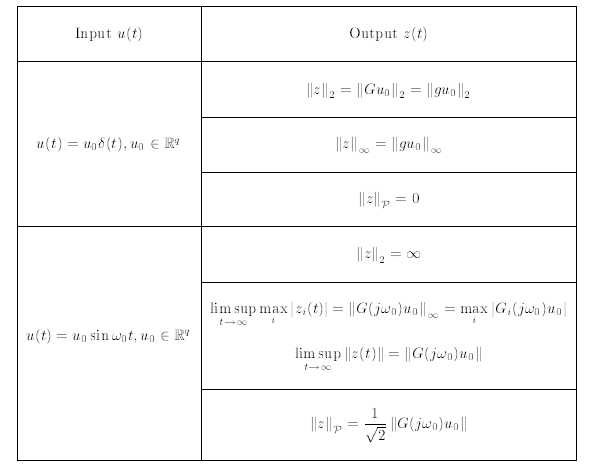
\includegraphics[scale = 0.9]{Control/Controlf1.png}
\end{figure}

Es interesante ver el significado de la tabla anterior desde el punto de vista del control. En nuestro foco de atención, asumimos que la señal de entrada $u(t)=u_0 \sin{\omega_0 t}$ es una perturbación o una señal de comando en el sistema realimentado, y la señal $z(t)$ es la señal de error. Entonces se dice que el sistema tiene un buen error de seguimiento si $z(t)$ es pequeña en algún sentido, por ejemplo, $\limsup_{t \to \infty}{||z(t)||}$. Note que

\begin{equation*}
    \limsup_{t \to \infty}{||z(t)||} = ||G(j \omega_0 )u_0||
\end{equation*}

para cualquier frecuencia dada $\omega_0$ y $u_0 \in \mathbb{R}^q$. Ahora si queremos seguir señales desde varios canales, esto es, si $u_0$ puede ser ecogido en cualquier direección, entonces se requeriría que $\bar{\sigma}( G (j \omega) )$ sea pequeño. Adicionalmente, si queremos seguir señales de muchas frecuencias distintas, entonces $\bar{\sigma}( G (j \omega) )$ deberá ser pequeño a todas esas frecuencias.\\

En la siguiente tabla se muestra la máxima ganancia posible cuando la señal de entrada no está dada como una señal fija.

\begin{figure}[H]
    \centering
    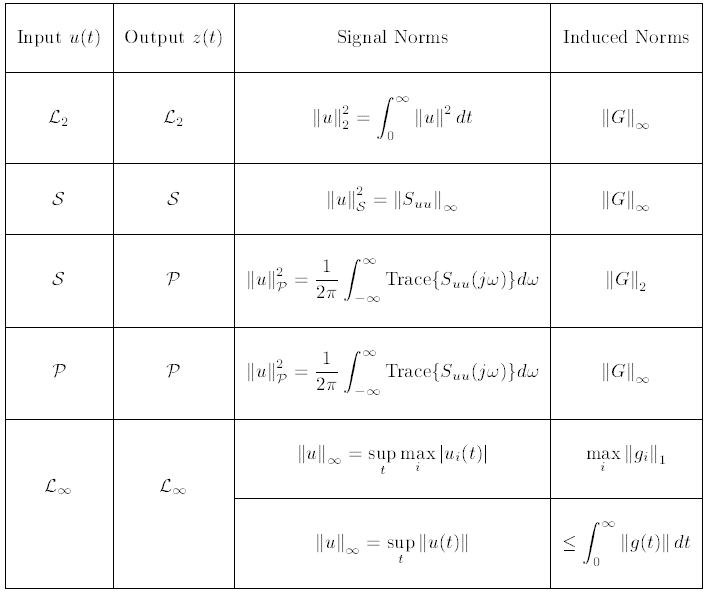
\includegraphics[scale = 0.85]{Control/controlf2.png}
\end{figure}


Derivemos algunos límites útiles para la norma $\mathcal{H}_\infty$ y la norma de $\mathcal{L}_1$ de un sistema estable, suponga que

\begin{equation*}
    G_1(s) = \left( \begin{tabular}{c|c}$A_1$&$B_1$\\\hline$C_1$&$D_1$\end{tabular} \right) \in \mathcal{R H}_\infty
\end{equation*}

es una realización balanceada, es decir, que $\Sigma = diag(\sigma_1,\sigma_2,\dots,\sigma_n) \geq 0$, con $\sigma_1 \geq \sigma_2 \geq \dots \geq \sigma_n \geq 0$ tal que

\begin{equation*}
    A \Sigma + \Sigma A^{*} + B \ B^{*} = 0
\end{equation*}


\begin{equation*}
    A^{*} \Sigma + \Sigma A + C^{*} \ C  = 0
\end{equation*}
entonces tenemos el siguiente teorema

\subsubsection{Teorema} 

\begin{equation*}
    \sigma_1 \leq ||G||_\infty \leq \int_{0}^{\infty} ||g(t)|| dt \leq 2 \sum_{i=1}^{n} \sigma_i
\end{equation*}

donde $g(t) = Ce^{At}B$

\begin{figure}[H]
    \centering
    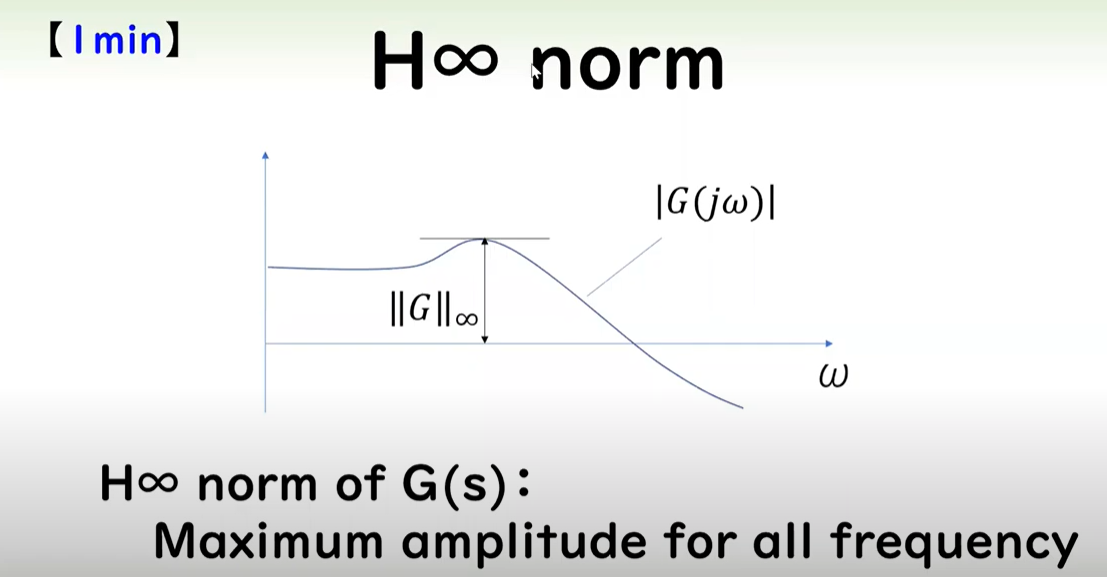
\includegraphics[scale = 0.5]{Control/controlf3.png}
\end{figure}


\section{Calculando las normas L2 y H2}

Sea $G(s) \in \mathcal{L}_2$, y recuerde que la norma $\mathcal{L}_2$ de $G$ se define como sigue

\begin{eqnarray*}
    ||G||_2 & := & \sqrt{\frac{1}{2 \pi} \int_{- \infty}^{\infty}\text{Tr}(G^{*}(j \omega) G(j \omega))d \omega} \\
    &=& ||g||_2 \\
    &=& \sqrt{\int_{- \infty}^{\infty}\text{Tr}(g^{*}(t) g(t))d \omega}
\end{eqnarray*}

donde $g(t)$ es el núcleo de convolución de $G$.

Es fácil de ver que la norma $\mathcal{L}_2$ es finita si y solo si la matriz de transferencia $G$ es estrictamente propia. Así vamos a asumir de manera general que la matriz es estrictamente propia. Una forma sencilla de calcular la norma $\mathcal{L}_2$ es usar integrales de contorno


\begin{equation*}
     ||G||_2^{2} = \frac{1}{2 \pi} \int_{- \infty}^{\infty}\text{Tr}(G^{*}(j \omega) G(j \omega))d \omega
\end{equation*}


\begin{equation*}
     ||G||_2^{2} = \frac{1}{2 \pi j} \oint \text{Tr}(G^{*}(s) G(s))d s
\end{equation*}

La anterior es una integral de contorno a lo largo del eje imaginario y al redededor del semicírculo infinito del semiplano izquierdo, la contribución a la integral de la sección de semicpirculo infinito es igual a cero dado que la matriz de transferencia es estrictamente propia. Por el teorema del residuo, $ ||G||_2^{2}$ es igual a la suma de los residuos de $\text{Tr}(G^{*}(s) G(s))$ en sus polos en el semiplano izquierdo.

Aunque la norma puede ser calculada en principio de su definición es más util en muchas aplicaciones tener una caracterización alternativa y tener ventajas de la s representaciones de espacio de estados de G. El cálculo de la norma $\mathcal{R H}_2$ de una matriz de transferencia es particularmente simple. \\

\paragraph{Lema} Considere la matriz de transferencia
\begin{equation*}
    G_1(s) = \left( \begin{tabular}{c|c}$A$&$B$\\\hline$C$&$0$\end{tabular} \right) 
\end{equation*}
Donde $A$ es estable. Entonces tenemos que 
\begin{equation*}
    ||G||_2^2 = \text{Tr}(B^{*} W_o B) = \text{Tr}(C W_c C^{*})
\end{equation*}
donde $W_o$ y $W_c$ son los gramianos de controlabilidad y observabilidad y se pueden obtener de las siguientes ecuaciones de Lyapunov
\begin{equation*}
    A W_c + W_c A^{*} + B B^{*} = 0
\end{equation*}
\begin{equation*}
    A^{*} W_o + W_o A + C^{*} C = 0
\end{equation*}


